\documentclass[conference,compsoc,final,a4paper]{IEEEtran}
\usepackage[utf8]{inputenx}
\linespread{1.25}


%% Bitte legen Sie hier den Titel und den Autor der Arbeit fest
\newcommand{\autoren}[0]{Kari, Jonas \newline Rittershofer, Daniel}

\newcommand{\dokumententitel}[0]{DevSecOps - Implementierung von Quality-Gates zur Förderung der Sicherheit von Software-Artefakten während der Entwicklung}

\input{preambel} % Weitere Einstellungen aus einer anderen Datei lesen

\begin{document}

% Titel des Dokuments
\title{\dokumententitel}

% Namen der Autoren
\author{
  \IEEEauthorblockN{\autoren}
  \IEEEauthorblockA{
    Hochschule Mannheim\\
    Fakultät für Informatik\\
    Paul-Wittsack-Str. 10,
    68163 Mannheim
    }
}

% Titel erzeugen
\maketitle
\thispagestyle{plain}
\pagestyle{plain}

% Eigentliches Dokument beginnt hier
% ----------------------------------------------------------------------------------------------------------

% Kurze Zusammenfassung des Dokuments
\begin{abstract}
In dieser Arbeit werden grundlegende Prinzipien von DevSecOps beschrieben und anhand von Implementierungen verdeutlicht. Der Schwerpunkt liegt dabei auf der Implementierung von Quality Gates. Insbesondere wird der Fokus auf das Dependency Scanning zur Identifikation bekannter Sicherheitslücken, sowie auf statische Code-Analyse, um potenzielle Fehler und Schwachstellen im Code frühzeitig zu erkennen, gelegt.
\end{abstract}

% Inhaltsverzeichnis erzeugen
{\small\tableofcontents}

% Abschnitte mit \section, Unterabschnitte mit \subsection und
% Unterunterabschnitte mit \subsubsection
% -------------------------------------------------------


% -------------------------------------------------------
\section{Entstehung von DevOps und der Weg zu DevSecOps}
In der heutigen Zeit gewinnt das DevOps-Prinzip im Softwareentwicklungszyklus zunehmend an Bedeutung. DevOps fördert die Integration von Entwicklung und Betrieb und verkürzt die bisherige Trennung zwischen diesen Bereichen. Dieser Ansatz wird durch das Prinzip "you build it, you run it" verkörpert, welches die Verantwortlichkeit für den gesamten Lebenszyklus einer Anwendung in die Hände der Entwickler legt.

Ein wesentlicher Aspekt dieser Integration ist die Sicherheit, die traditionell als separater Schritt behandelt wurde. Der "shift left" Ansatz integriert Sicherheitsaspekte frühzeitig und kontinuierlich in den Softwareentwicklungsprozess. Dies bedeutet, dass Sicherheitsmaßnahmen nicht nur in der Entwicklungsphase, sondern auch während des Betriebs berücksichtigt werden müssen.

In dieser Arbeit liegt der Schwerpunkt auf der Implementierung von Quality Gates, die darauf abzielen, die Sicherheit von Software zu erhöhen. Insbesondere wird der Fokus auf das Dependency Scanning zur Identifikation bekannter Sicherheitslücken und die statische Code-Analyse gelegt, um potenzielle Fehler und Schwachstellen im Code frühzeitig zu erkennen.

Durch diese Maßnahmen wird nicht nur die Sicherheit der Software verbessert, sondern auch die Effizienz des gesamten Entwicklungsprozesses gesteigert. Die Bedeutung dieser Ansätze wird im Kontext moderner Softwareentwicklung erläutert und durch praxisnahe Beispiele und Fallstudien untermauert.


Diese Arbeit richtet sich an Software-Entwickler und IT-Fachleute, die DevOps und DevSecOps einführen möchten. Ziel ist es, die Sicherheit und Qualität ihrer Software-Releases zu verbessern. Leser sollten grundlegendes Wissen über Softwareentwicklung und IT-Betrieb haben und daran interessiert sein, Sicherheits- und Qualitätsstrategien sowie Security-Gates in ihren Entwicklungsprozess zu integrieren. Die Arbeit bietet anhand von zwei Beispielen eine Implementierung sowie Best Practices, um eine sichere und effiziente
\section{Historische Entwicklung von DevOps zu DevSecOps}
Dieses Kapitel zeigt die Entstehung der DevOps-Kultur auf und wie der logische Schritt zu DevSecOps vollzogen wurde.

\subsection{Entstehung von DevOps und der Weg zu DevSecOps}
Der Begriff DevOps entstand Ende der 2000er Jahre und beschreibt die engere Zusammenarbeit von Software-Entwicklung und IT-Betrieb. In der Vergangenheit – und teilweise auch heute noch – führten die Kluft zwischen Abteilungen und unklare Zuständigkeiten oft zu Problemen, die erst dann sichtbar wurden, wenn eine Abteilung, die nicht in die Entwicklung involviert war, eine Software oder ein Softwaresystem mit meist manuellen Schritten in den Produktivbetrieb übernehmen sollte. Durch das DevOps-Prinzip können solche Probleme frühzeitig erkannt werden, insbesondere durch ein T-Shaped-Entwicklungsteam, in dem auch Kenntnisse im Betrieb von Software vorhanden sind.

DevOps ist als eine Kultur und Praxis zu verstehen, die Entwicklung und Betrieb integriert. Ziel ist es, durch automatisierte Prozesse und verbesserte Zusammenarbeit eine qualitativ hochwertige und reproduzierbar betreibbare Software schneller bereitzustellen.

\subsection{TBD: Zusammenarbeit zwischen Entwicklung und Betrieb}
Traditionell arbeiteten Entwicklung und Betrieb isoliert, was zu Kommunikationsproblemen und Verzögerungen führte. DevOps fördert die enge Zusammenarbeit beider Teams, um schnell auf Marktveränderungen zu reagieren und die Softwarequalität zu verbessern.


\subsection{TBD: Prinzipien der kontinuierlichen Integration und kontinuierlichen Bereitstellung (CI/CD)}
Kontinuierliche Integration (CI): Entwickler integrieren regelmäßig ihren Code in ein zentrales Repository, gefolgt von automatisierten Builds und Tests, um Fehler frühzeitig zu erkennen und zu beheben.

Kontinuierliche Bereitstellung (CD): Automatisiert die Bereitstellung von Softwareänderungen in verschiedene Umgebungen, sodass jede erfolgreiche Änderung schnell und zuverlässig an Endnutzer ausgeliefert werden kann.

\section{Integration von Statischer Code Analyse in den DevOps-Zyklus}
In diesem Kapitel wird anhand von statischer Code-Analyse und Dependency Scanning aufgezeigt, wie Sicherheitslücken erkannt und behoben werden können, bevor diese in für den Produktionsbetrieb freigegebenen Releases veröffentlicht und in Betrieb genommen werden.

\subsection{Nutzung von Statischer Code Analyse}
Die Nutzung von statischer Code-Analyse ist ein essenzieller Bestandteil moderner Softwareentwicklungsprozesse, um die Codequalität und Sicherheit zu gewährleisten. Es gibt eine Vielzahl von Tools zur Durchführung dieser Analysen, darunter SonarQube, ESLint, Pylint und Coverity. Die Autoren dieses Kapitels fokussieren sich auf die Verwendung von SonarQube, basierend auf ihrer umfangreichen Erfahrung und den Vorteilen, die SonarQube bietet. SonarQube wird häufig gewählt, weil es eine umfassende Analyse für eine Vielzahl von Programmiersprachen bietet und sich nahtlos in verschiedene CI/CD-Tools integrieren lässt.

Durch die Integration von SonarQube in den CI/CD-Prozess kann diese Analyse automatisiert und kontinuierlich durchgeführt werden. Innerhalb des GitFlow-Workflows ermöglicht es die Einrichtung von Quality Gates in SonarQube, die spezifische Richtlinien und Kriterien definieren, die der Code erfüllen muss. Wenn diese Quality Gates durch die in SonarQube hinterlegten Policies fehlschlagen, wird der Build-Prozess unterbrochen und ein Merge in ein Release verhindert. Dadurch wird sichergestellt, dass nur qualitativ hochwertiger und sicherer Code in die Produktionsumgebung gelangt, wodurch das Risiko von Sicherheitslücken und anderen Problemen erheblich reduziert wird.

\subsubsection{Übersicht der Tools zur statischen Code Analyse}

Es gibt eine Vielzahl von Tools, die zur statischen Code Analyse eingesetzt werden können. Die folgende Tabelle gibt eine Übersicht über einige gängige Tools:

\begin{table*}[h!]
\centering
\begin{tabular}{|l|l|l|l|}
\hline
\textbf{Tool} & \textbf{Programmiersprachen} & \textbf{Lizenz} & \textbf{Besonderheiten} \\ \hline
SonarQube & Mehrere & Open Source & Umfangreiche Analyse, Integration in CI/CD \\ \hline
ESLint & JavaScript, TypeScript & Open Source & Speziell für JavaScript, konfigurierbar \\ \hline
Checkmarx & Mehrere & Proprietär & Fokus auf Sicherheit \\ \hline
PMD & Java, Apex & Open Source & Regelbasierte Analyse \\ \hline
Bandit & Python & Open Source & Sicherheitsanalyse für Python \\ \hline
\end{tabular}
\caption{Übersicht von Tools zur statischen Code Analyse}
\label{tab:static_code_analysis_tools}
\end{table*}

\subsubsection{Integration von SonarQube in die CI/CD-Pipeline}

SonarQube ist ein weit verbreitetes Tool zur statischen Code Analyse, das eine nahtlose Integration in CI/CD-Pipelines unterstützt. Im Folgenden wird gezeigt, wie SonarQube mit GitHub Actions integriert werden kann, um eine automatisierte Analyse des Codes durchzuführen.

\paragraph{Einrichtung von SonarQube}

SonarQube kann auf verschiedene Weise eingerichtet werden: lokal, als SaaS oder on-premise. Eine einfache Möglichkeit zur lokalen Einrichtung bietet Docker. Die folgende \texttt{docker-compose.yml} Datei zeigt ein Beispiel:

\begin{lstlisting}
version: '3'

services:
  sonarqube:
    image: sonarqube:latest
    ports:
      - "9000:9000"
    environment:
      SONARQUBE_JDBC_URL: jdbc:postgresql://db:5432/sonarqube
      SONARQUBE_JDBC_USERNAME: sonar
      SONARQUBE_JDBC_PASSWORD: sonar
  db:
    image: postgres:latest
    environment:
      POSTGRES_USER: sonar
      POSTGRES_PASSWORD: sonar
      POSTGRES_DB: sonarqube
\end{lstlisting}

\paragraph{Integration mit verschiedenen CI/CD-Tools}

Neben GitHub Actions kann SonarQube auch in andere CI/CD-Tools integriert werden, wie z.B. GitLab CI/CD und Azure DevOps.


\paragraph{Konfiguration der GitHub Actions Workflow-Datei}

Erstellen Sie im Wurzelverzeichnis Ihres Repositories eine Datei namens \texttt{.github/workflows/sonarqube.yml} mit folgendem Inhalt:

\begin{lstlisting}
name: SonarQube Analysis

on:
  push:
    branches:
      - main
      - develop
  pull_request:
    branches:
      - main
      - develop

jobs:
  sonarQube:
    runs-on: ubuntu-latest

    steps:
    - name: Check out repository
      uses: actions/checkout@v2

    - name: Set up JDK 11
      uses: actions/setup-java@v1
      with:
        java-version: '11'

    - name: Cache SonarQube packages
      uses: actions/cache@v2
      with:
        path: ~/.sonar/cache
        key: ${{ runner.os }}-sonar-cache
        restore-keys: ${{ runner.os }}-sonar-cache

    - name: Install dependencies
      run: ./gradlew build -x test

    - name: Run SonarQube analysis
      env:
        SONAR_TOKEN: ${{ secrets.SONAR_TOKEN }}
      run: ./gradlew sonarqube -Dsonar.projectKey=my_project_key -Dsonar.host.url=https://sonarqube.mycompany.com -Dsonar.login=${{ secrets.SONAR_TOKEN }}
\end{lstlisting}

\paragraph{Branch-Regeln und Merge-Policies}

Um sicherzustellen, dass nur Code, der den definierten Sicherheitsstandards entspricht, in die Haupt-Branches integriert wird, können Branch-Regeln und Merge-Policies in GitHub konfiguriert werden. Hierbei wird beispielsweise das Mergen von Branches blockiert, die den OWASP-Standards in SonarQube nicht entsprechen.

\begin{itemize}
    \item Gehe zu den Einstellungen des Repositories auf GitHub.
    \item Wähle \textit{Branches} und dann \textit{Branch protection rules}.
    \item Erstelle eine neue Regel für den \textit{main} und \textit{develop} Branch.
    \item Aktiviere die Option \textit{Require status checks to pass before merging} und füge den SonarQube-Status hinzu.
\end{itemize}

\subsubsection{Erstellung eigener Policies und Verwendung von OWASP Policies}

SonarQube bietet die Möglichkeit, eigene Quality Gates und Regeln zu definieren. Diese können auf verschiedene Metriken und Bedingungen basieren, um sicherzustellen, dass der Code bestimmten Standards entspricht.

\paragraph{Beispiele für OWASP Policies in SonarQube}

SonarQube wird mit vordefinierten OWASP Policies ausgeliefert, die häufige Sicherheitslücken identifizieren. Dazu gehören:

\begin{itemize}
    \item \textbf{SQL Injection}: Überprüft auf Anfälligkeiten für SQL-Injection-Angriffe.
    \item \textbf{Cross-Site Scripting (XSS)}: Erkennt potenzielle XSS-Schwachstellen.
    \item \textbf{Insecure Deserialization}: Identifiziert unsichere Deserialisierungen.
\end{itemize}

\subsubsection{Beispielkonfiguration und Demonstration}

\subsubsection{Erstellung und Verwendung des GitFlow-Modells}

Das GitFlow-Modell ist ein weit verbreitetes Workflow-Modell, das die Arbeit mit Feature-Branches und Release-Branches strukturiert. Es wird folgendermaßen implementiert:

\begin{itemize}
    \item \textbf{main}: Enthält den Produktionscode.
    \item \textbf{develop}: Basis für neue Features.
    \item \textbf{feature-branches}: Abgeleitet von \textit{develop}, für die Entwicklung neuer Features.
    \item \textbf{release-branches}: Vorbereitung für neue Releases.
    \item \textbf{hotfix-branches}: Dringende Korrekturen auf dem \textit{main}-Branch.
\end{itemize}

\paragraph{Workflow-Illustration}

\begin{figure*}[h!]
\centering
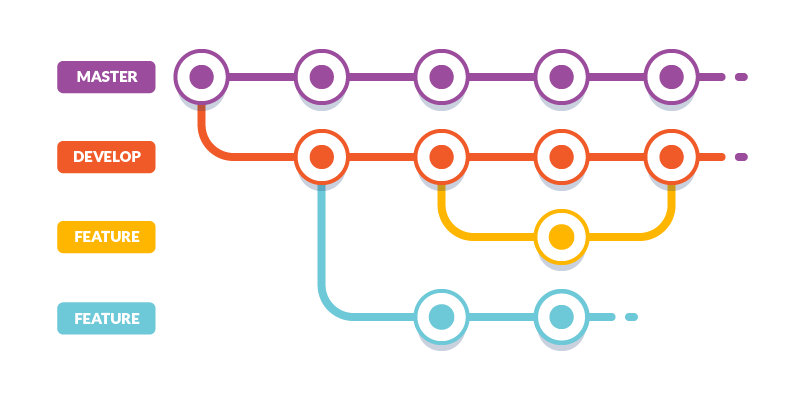
\includegraphics[width=\textwidth]{img/gitflow_workflow.png}
\caption{Illustration des GitFlow-Modells}
\label{fig:gitflow}
\end{figure*}

\paragraph{Beispielhafte Umsetzung in GitHub}

\begin{enumerate}
    \item Forke das Repository und erstelle einen neuen Branch: \texttt{git checkout -b feature/new-feature develop}
    \item Implementiere das neue Feature und pushe die Änderungen: \texttt{git push origin feature/new-feature}
    \item Öffne einen Pull Request von \texttt{feature/new-feature} nach \texttt{develop}.
    \item Die CI/CD-Pipeline führt die statische Code Analyse mit SonarQube durch.
    \item Bestehen alle Checks, kann der Branch gemerged werden.
\end{enumerate}

\paragraph{Screenshots und Ergebnisinterpretation}

Fügen Sie hier passende Screenshots ein, die die Ergebnisse der SonarQube-Analyse und den Workflow der GitHub Actions demonstrieren.

\begin{figure*}[h!]
\centering
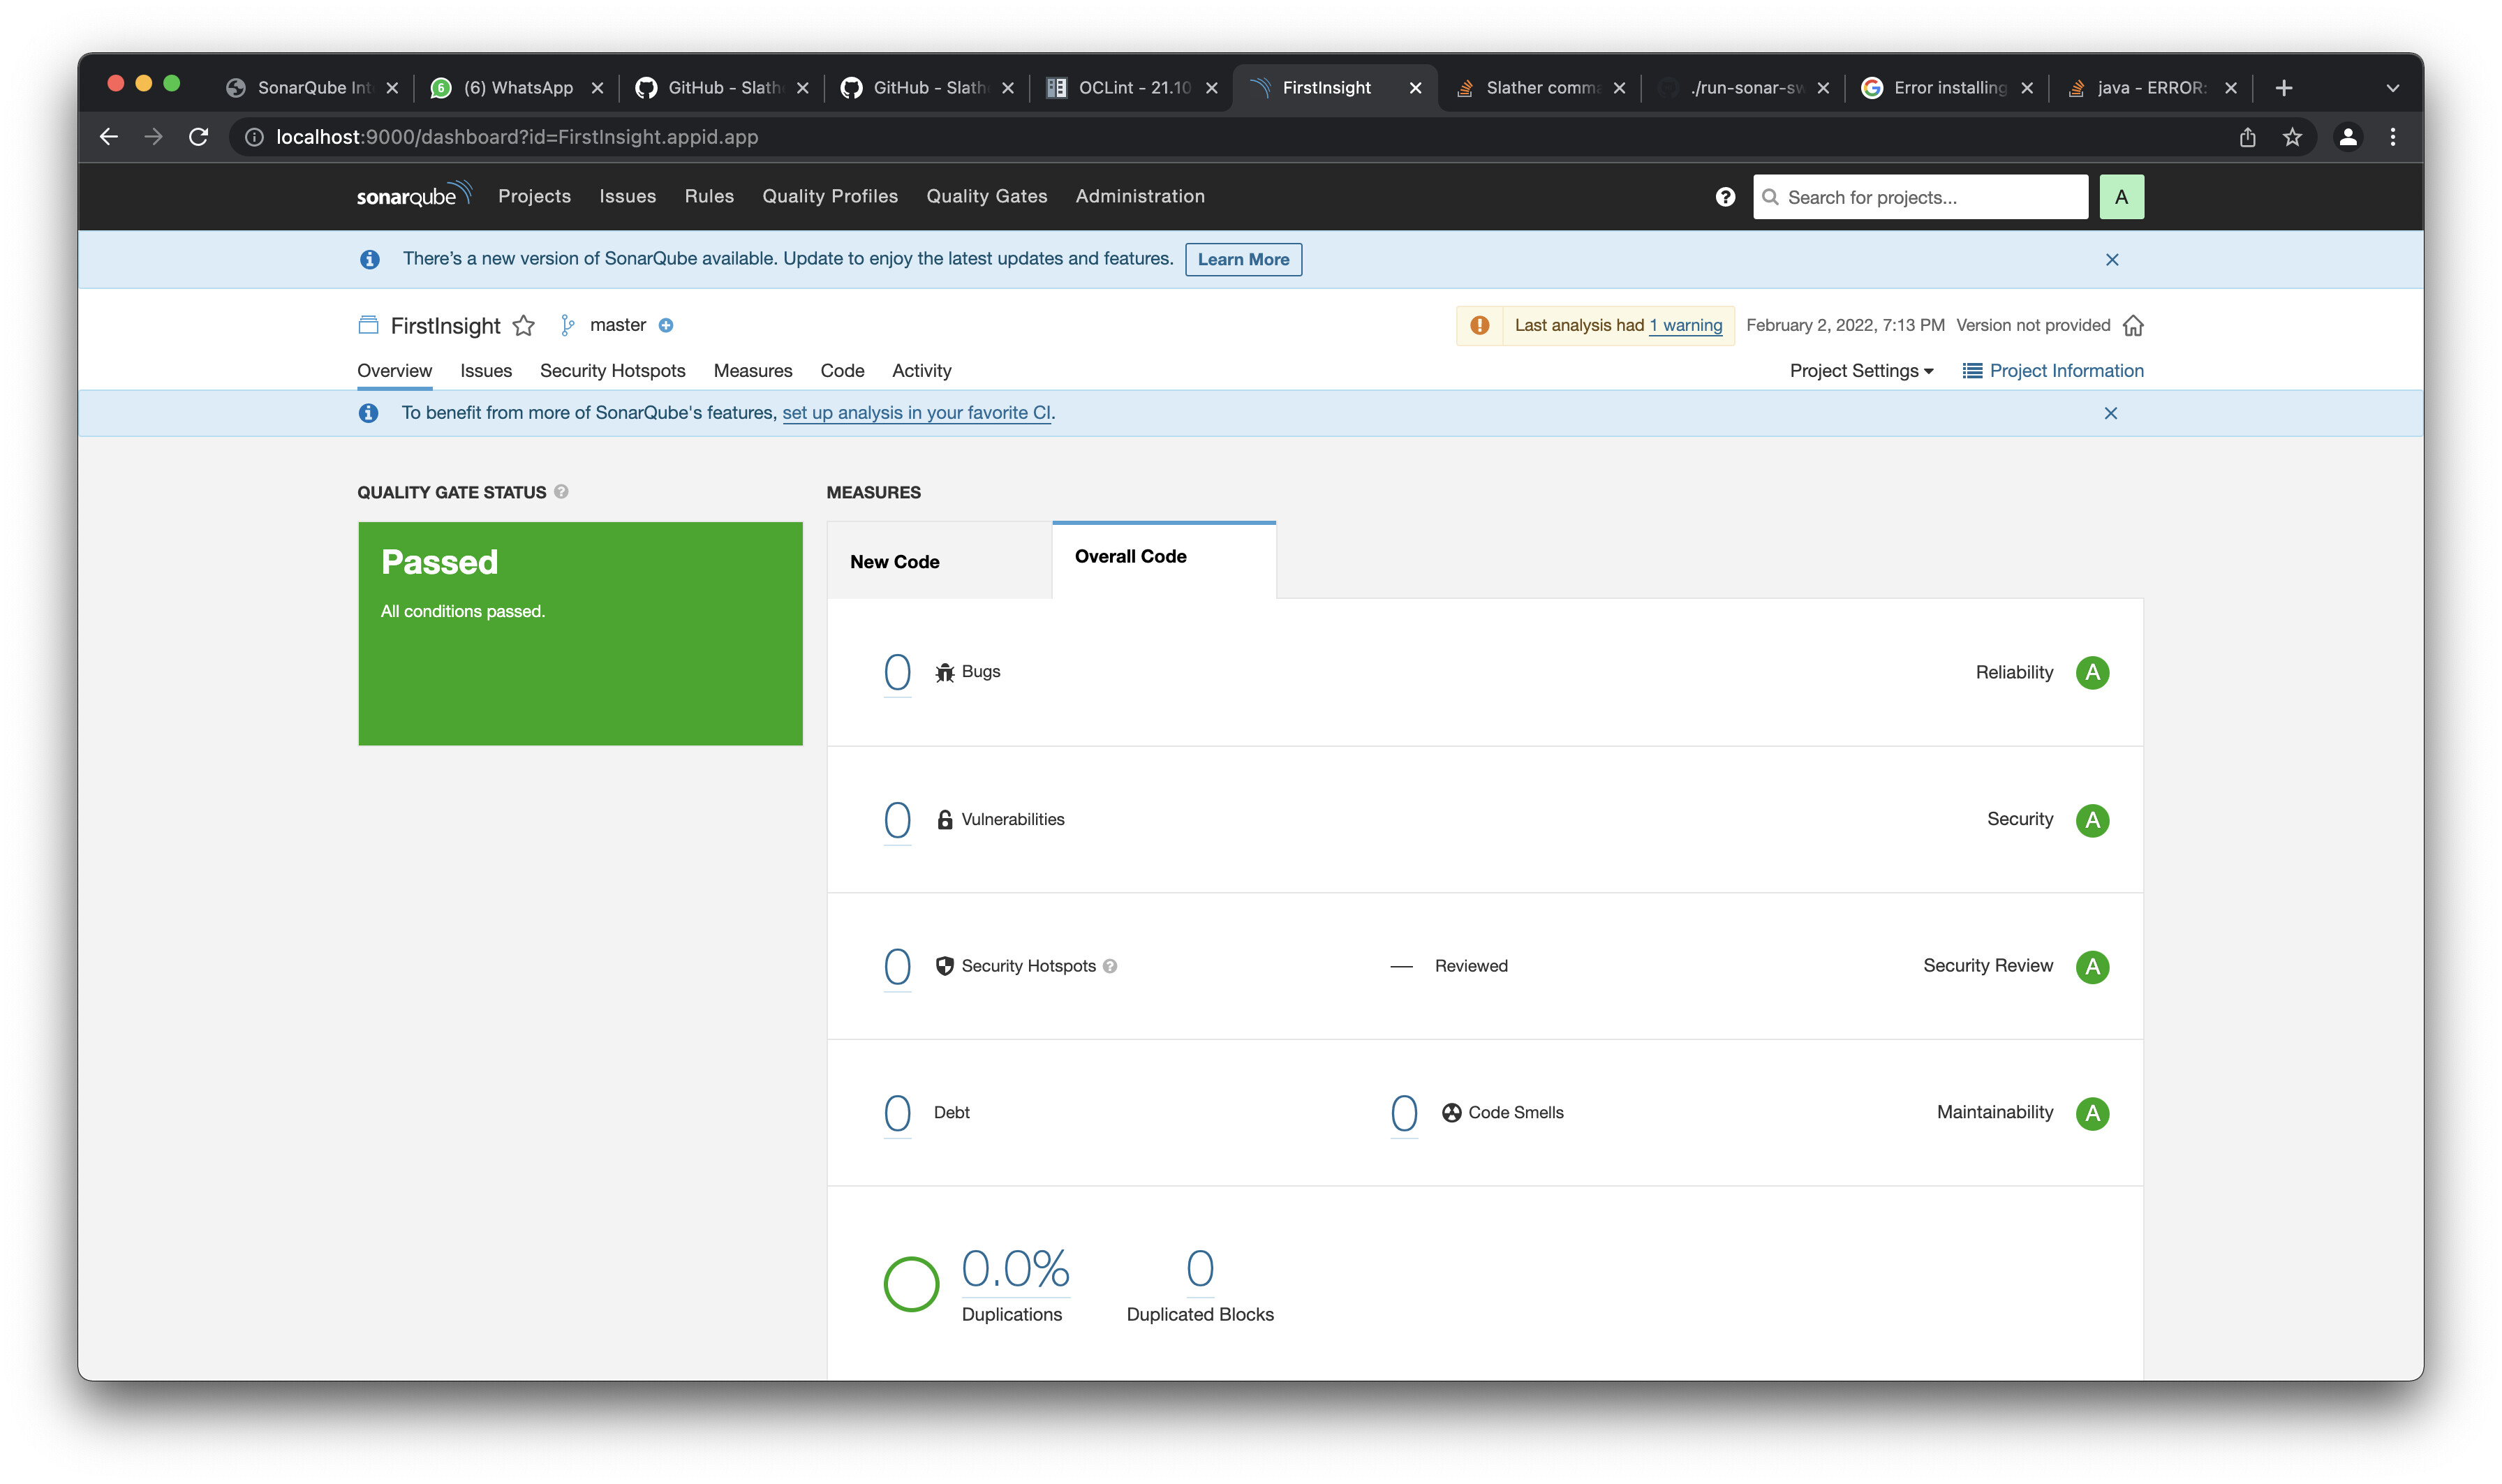
\includegraphics[width=\textwidth]{img/sonarqube_results.jpeg}
\caption{Ergebnisse der SonarQube-Analyse}
\label{fig:sonarqube_results}
\end{figure*}

\begin{figure*}[h!]
\centering
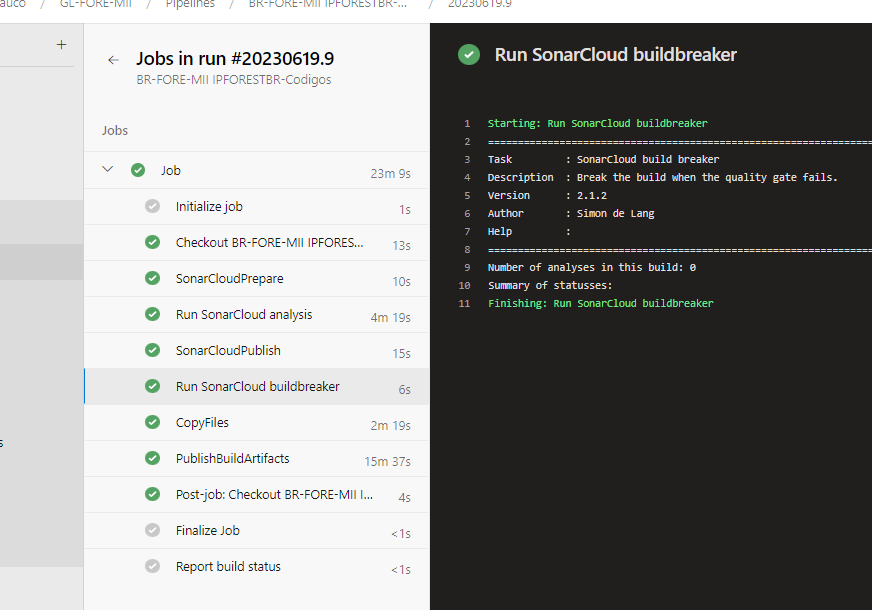
\includegraphics[width=\textwidth]{img/github_actions_failed_quality_gate.png}
\caption{GitHub Actions Workflow mit fehlgeschlagenem Quality Gate}
\label{fig:github_actions_failed_quality_gate}
\end{figure*}

\subsubsection{Metriken in SonarQube}

SonarQube bietet eine Vielzahl von Metriken, um die Qualität und Sicherheit des Codes zu bewerten. Zu den wichtigsten Metriken gehören:

\begin{itemize}
    \item \textbf{Bugs}: Fehler im Code, die potenziell zu falschem Verhalten führen.
    \item \textbf{Code Smells}: Hinweise auf Bereiche des Codes, die verbessert werden können.
    \item \textbf{Vulnerabilities}: Sicherheitslücken, die ausgenutzt werden könnten.
    \item \textbf{Coverage}: Prozentsatz des Codes, der durch Tests abgedeckt ist.
    \item \textbf{Duplications}: Anteil des Codes, der dupliziert ist.
\end{itemize}

\paragraph{Beispielhaftes SonarQube Dashboard}

\begin{figure*}[h!]
\centering
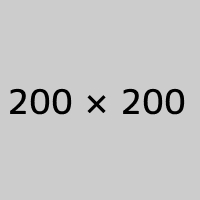
\includegraphics[width=\textwidth]{img/sonarqube_dashboard.png}
\caption{Beispiel eines SonarQube Dashboards}
\label{fig:sonarqube_dashboard}
\end{figure*}

\subsubsection{Schlussfolgerungen und Best Practices}

Die Integration von statischer Code Analyse in den CI/CD-Prozess verbessert nicht nur die Codequalität, sondern trägt auch zur Erhöhung der Sicherheit bei. Durch den Einsatz von Tools wie SonarQube in Kombination mit GitHub Actions, GitLab CI/CD oder Azure DevOps und strikten Branch-Regeln können potenzielle Schwachstellen frühzeitig erkannt und behoben werden.

\section{Integration von Dependency Scanning und Überprüfung auf Sicherheitslücken in den DevOps-Zyklus}
In diesem Kapitel wird anhand von Dependency Scanning und der Überprüfung auf Sicherheitslücken aufgezeigt, wie Sicherheitslücken in Abhängigkeiten erkannt und behoben werden können, bevor diese in für den Produktionsbetrieb freigegebenen Releases veröffentlicht und in Betrieb genommen werden.

\subsection{Nutzung von Dependency Scanning}
Dependency Scanning und die Überprüfung auf Sicherheitslücken sind kritische Schritte im Softwareentwicklungsprozess, um sicherzustellen, dass alle verwendeten Bibliotheken und Abhängigkeiten sicher und auf dem neuesten Stand sind. Es gibt mehrere Tools, die für diesen Zweck verwendet werden können, darunter Sonatype Nexus IQ, Snyk und OWASP Dependency-Check. Die Autoren dieses Kapitels fokussieren sich auf die Verwendung von Sonatype Nexus IQ aufgrund ihrer umfassenden Erfahrung und der weitreichenden Fähigkeiten dieses Tools.

\subsubsection{Übersicht ähnlicher Produkte}

Es gibt verschiedene Tools, die zur Überprüfung von Abhängigkeiten auf Sicherheitslücken verwendet werden können. Die folgende Tabelle gibt eine Übersicht über einige gängige Tools:

\begin{table*}[h!]
\centering
\begin{tabular}{|l|l|l|l|}
\hline
\textbf{Tool} & \textbf{Programmiersprachen} & \textbf{Lizenz} & \textbf{Besonderheiten} \\ \hline
Sonatype Nexus IQ & Mehrere & Proprietär & Umfassende Sicherheitsanalyse, Policy Enforcement \\ \hline
Snyk & Mehrere & Proprietär & Echtzeit-Schwachstellenüberprüfung, Entwicklungsintegration \\ \hline
OWASP Dependency-Check & Mehrere & Open Source & Fokus auf bekannte Sicherheitslücken \\ \hline
WhiteSource & Mehrere & Proprietär & Automatisierte Open-Source-Sicherheit und Compliance \\ \hline
Black Duck & Mehrere & Proprietär & Umfassende Open-Source-Risikoanalyse \\ \hline
\end{tabular}
\caption{Übersicht von Tools zur Überprüfung von Abhängigkeiten}
\label{tab:dependency_scanning_tools}
\end{table*}

\subsubsection{Funktionsweise von Sonatype Nexus IQ}

Sonatype Nexus IQ ist ein fortschrittliches Tool zur Analyse von Abhängigkeiten und zur Erkennung von Sicherheitslücken. Es arbeitet durch:

\begin{itemize}
    \item \textbf{Scannen der Abhängigkeiten}: Analysiert alle im Projekt verwendeten Abhängigkeiten.
    \item \textbf{Abgleich mit Datenbanken}: Vergleicht Abhängigkeiten mit bekannten Schwachstellen in öffentlichen und privaten Datenbanken.
    \item \textbf{Policy Enforcement}: Überprüft Abhängigkeiten gegen vordefinierte Sicherheitsrichtlinien und Policies.
    \item \textbf{Berichterstellung}: Generiert Berichte und Warnungen über erkannte Sicherheitslücken und Risiken.
\end{itemize}

\begin{figure*}[h!]
\centering
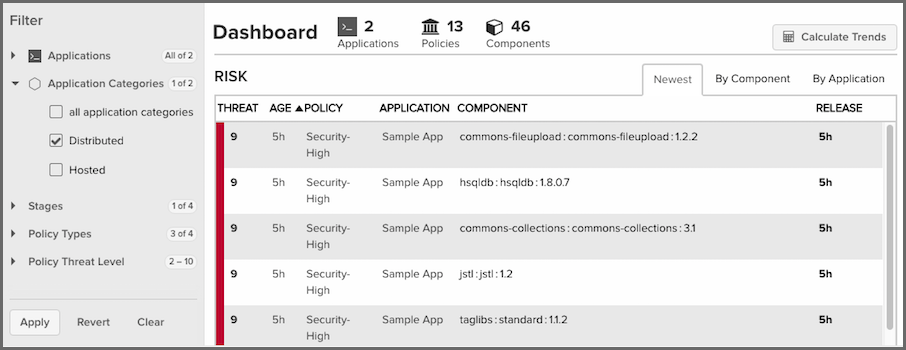
\includegraphics[width=\textwidth]{nexusiq_dashboard.png}
\caption{Beispiel eines Sonatype Nexus IQ Dashboards}
\label{fig:nexusiq_dashboard}
\end{figure*}

\subsubsection{Vorteile von Sonatype Nexus IQ}

Die Verwendung von Sonatype Nexus IQ bietet zahlreiche Vorteile:

\begin{itemize}
    \item \textbf{Umfassende Sicherheitsanalyse}: Erkennt eine Vielzahl von Schwachstellen in Abhängigkeiten.
    \item \textbf{Automatisierte Policy Enforcement}: Stellt sicher, dass nur sichere und konforme Abhängigkeiten verwendet werden.
    \item \textbf{Integration in CI/CD}: Kann nahtlos in bestehende CI/CD-Pipelines integriert werden.
    \item \textbf{Detaillierte Berichte}: Bietet umfangreiche Berichte und Dashboards zur Überwachung der Sicherheit.
    \item \textbf{Regelmäßige Updates}: Erhält kontinuierliche Updates zu neuen Sicherheitslücken und Bedrohungen.
\end{itemize}

\subsubsection{Beispiel Implementierung für GitHub Actions}

Ein typisches Setup für die Integration von Sonatype Nexus IQ in GitHub Actions könnte wie folgt aussehen:

\paragraph{Einrichtung der GitHub Actions Workflow-Datei}

Erstellen Sie im Wurzelverzeichnis Ihres Repositories eine Datei namens \texttt{.github/workflows/nexus-iq.yml} mit folgendem Inhalt:

\begin{lstlisting}
name: Nexus IQ Analysis

on:
  push:
    branches:
      - main
      - develop
  pull_request:
    branches:
      - main
      - develop

jobs:
  nexusIQ:
    runs-on: ubuntu-latest

    steps:
    - name: Check out repository
      uses: actions/checkout@v2

    - name: Set up JDK 11
      uses: actions/setup-java@v1
      with:
        java-version: '11'

    - name: Cache Nexus IQ packages
      uses: actions/cache@v2
      with:
        path: ~/.nexus/cache
        key: ${{ runner.os }}-nexus-cache
        restore-keys: ${{ runner.os }}-nexus-cache

    - name: Install dependencies
      run: ./gradlew build -x test

    - name: Run Nexus IQ analysis
      env:
        NEXUS_IQ_URL: ${{ secrets.NEXUS_IQ_URL }}
        NEXUS_IQ_USERNAME: ${{ secrets.NEXUS_IQ_USERNAME }}
        NEXUS_IQ_PASSWORD: ${{ secrets.NEXUS_IQ_PASSWORD }}
      run: ./gradlew nexusIqScan -Dsonar.projectKey=my_project_key -Dsonar.host.url=${{ secrets.NEXUS_IQ_URL }} -Dsonar.login=${{ secrets.NEXUS_IQ_USERNAME }} -Dsonar.password=${{ secrets.NEXUS_IQ_PASSWORD }}
\end{lstlisting}

\subsubsection{Integration in den GitFlow}

Die Integration von Dependency Scanning in den GitFlow-Prozess folgt einem ähnlichen Muster wie bei der statischen Code Analyse:

\begin{itemize}
    \item \textbf{Feature-Branches}: Scannen der Abhängigkeiten während der Entwicklung neuer Features.
    \item \textbf{Develop-Branch}: Regelmäßiges Scannen vor dem Mergen von Feature-Branches.
    \item \textbf{Release-Branches}: Finales Scannen vor der Freigabe neuer Releases.
    \item \textbf{Hotfix-Branches}: Schnelles Scannen bei dringenden Fehlerbehebungen.
\end{itemize}

\paragraph{Beispielhafte Umsetzung in GitHub}

\begin{enumerate}
    \item Forke das Repository und erstelle einen neuen Branch: \texttt{git checkout -b feature/new-feature develop}
    \item Implementiere das neue Feature und pushe die Änderungen: \texttt{git push origin feature/new-feature}
    \item Öffne einen Pull Request von \texttt{feature/new-feature} nach \texttt{develop}.
    \item Die CI/CD-Pipeline führt das Dependency Scanning mit Sonatype Nexus IQ durch.
    \item Bestehen alle Checks, kann der Branch gemerged werden.
\end{enumerate}

\subsubsection{Sicherheitsgewinn durch Dependency Scanning}

Die Integration von Dependency Scanning und der Überprüfung auf Sicherheitslücken in den CI/CD-Prozess bietet erhebliche Sicherheitsvorteile:

\begin{itemize}
    \item \textbf{Früherkennung von Sicherheitslücken}: Sicherheitslücken in Abhängigkeiten werden frühzeitig erkannt und können behoben werden, bevor sie in die Produktionsumgebung gelangen.
    \item \textbf{Kontinuierliche Überwachung}: Durch kontinuierliches Scannen werden neue Schwachstellen sofort erkannt.
    \item \textbf{Compliance und Sicherheit}: Durchsetzen von Sicherheitsrichtlinien und Compliance-Anforderungen.
\end{itemize}

\subsubsection{Warnhinweise und Einschränkungen}

Es ist wichtig zu beachten, dass trotz der Verwendung von Tools wie Sonatype Nexus IQ Sicherheitslücken in Abhängigkeiten dennoch vorhanden sein können. Entwickler sollten sich dessen bewusst sein und folgende Vorsichtsmaßnahmen treffen:

\begin{itemize}
    \item \textbf{Regelmäßige Updates}: Stellen Sie sicher, dass alle Abhängigkeiten regelmäßig auf die neuesten Versionen aktualisiert werden.
    \item \textbf{Manuelle Überprüfungen}: Ergänzen Sie automatisierte Scans durch manuelle Überprüfungen und Sicherheitsaudits.
    \item \textbf{Bewusstsein und Schulung}: Schulen Sie das Entwicklungsteam in Best Practices der sicheren Softwareentwicklung.
    \item \textbf{Kontinuierliche Verbesserung}: Passen Sie Sicherheitsrichtlinien und -prozesse kontinuierlich an neue Bedrohungen und Schwachstellen an.
\end{itemize}

\subsubsection{Details zu OWASP}

Die Open Web Application Security Project (OWASP) bietet eine Vielzahl von Ressourcen zur Verbesserung der Software-Sicherheit. Das OWASP Top Ten Projekt ist eine jährlich aktualisierte Liste der am häufigsten auftretenden und kritischsten Sicherheitsrisiken für Webanwendungen. Einige der in Sonatype Nexus IQ integrierten OWASP-Regeln umfassen:

\begin{itemize}
    \item \textbf{Injection}: Schutz vor verschiedenen Injektionstypen, einschließlich SQL-Injection.
    \item \textbf{Broken Authentication}: Überprüfung auf Schwachstellen in der Authentifizierung.
    \item \textbf{Sensitive Data Exposure}: Sicherstellung der Verschlüsselung sensibler Daten.
    \item \textbf{XML External Entities (XXE)}: Erkennung von Schwachstellen, die durch externe XML-Entitäten verursacht werden.
    \item \textbf{Broken Access Control}: Verhinderung von unbefugtem Zugriff auf Ressourcen.
\end{itemize}

\subsubsection{Schlussfolgerungen und Best Practices}

Die Integration von Dependency Scanning in den CI/CD-Prozess verbessert nicht nur die Sicherheit der Software, sondern trägt auch zur Einhaltung von Compliance-Richtlinien bei. Tools wie Sonatype Nexus IQ bieten umfassende Analysen und automatisierte Policy Enforcement, um Sicherheitslücken frühzeitig zu erkennen und zu beheben. Es ist jedoch entscheidend, Sicherheitsmaßnahmen kontinuierlich zu überwachen und anzupassen, um den höchsten Sicherheitsstandard zu gewährleisten.
\section{Fazit}
Die Implementierung von statischer Code-Analyse und Dependency Scanning in den CI/CD-Prozess ist von entscheidender Bedeutung für die Sicherstellung der Codequalität und -sicherheit. Durch den Einsatz von SonarQube und Sonatype Nexus IQ können Entwickler frühzeitig potenzielle Probleme und Sicherheitslücken identifizieren und beheben. Die kontinuierliche Überprüfung und Durchsetzung von Qualitäts- und Sicherheitsrichtlinien tragen dazu bei, dass nur geprüfter und sicherer Code in die Produktionsumgebung gelangt. Die Anpassung der Berechtigungen für Release-Branches und die Einrichtung von automatisierten Workflows in GitHub Actions sind wichtige Schritte, um einen reibungslosen und sicheren Entwicklungsprozess zu gewährleisten. Letztendlich führen diese Maßnahmen zu einer höheren Softwarequalität, die den Anforderungen moderner Anwendungen gerecht wird.




% -------------------------------------------------------







% --------------------------------------------------------------------
\section*{Abkürzungen}
\addcontentsline{toc}{section}{Abkürzungen}

% Die längste Abkürzung wird in die eckigen Klammern
% bei \begin{acronym} geschrieben, um einen hässlichen
% Umbruch zu verhindern
% Sie müssen die Abkürzungen selbst alphabetisch sortieren!
\begin{acronym}[IEEE]
\acro{A2A}{Application-to-Application}
\acro{ABK}{Abkürzung}
\acro{ACL}{Acess Control List}
\acro{ACM}{Association of Computing Machinery}
\acro{AES}{Advanced Encryption Standard}
\acro{IEEE}{Institute of Electrical and Electronics Engineers}
\acro{ISO}{International Organization for Standardization}
\acro{PDF}{Portable Document Format}
\end{acronym}

% Literaturverzeichnis
\addcontentsline{toc}{section}{Literatur}
\printbibliography
\end{document}
